\documentclass[11pt,a4paper]{article}
\usepackage[utf8]{inputenc}
\usepackage[T1]{fontenc}
\usepackage[spanish,es-noshorthands]{babel}
\usepackage{lmodern}
\usepackage[margin=2.4cm]{geometry}
\usepackage{graphicx}
\usepackage{amsmath}
\usepackage{booktabs}
\usepackage{caption}
\usepackage{float}
\usepackage[table]{xcolor}
\usepackage[hidelinks]{hyperref}

\graphicspath{{../imagenes/}}
\captionsetup{font=small,labelfont=bf}
\setlength{\parskip}{0.45em}
\setlength{\parindent}{0pt}

\title{\vspace{-1.5cm}Avance sobre la pauta del 28 de septiembre}
\author{Javiera Palominos Clarke}
\date{26 de octubre de 2026}

\begin{document}
\maketitle
\vspace{-0.8cm}

Este documento reporta los seis puntos de la reunión del 28 de septiembre. Están todos
cerrados. Además se detectó y corrigió un error metodológico que afectaba cifras ya
reportadas, y el punto 5 derivó en un hallazgo sobre la representación que terminó siendo
el resultado más relevante del conjunto.

\begin{table}[H]
\centering
\small
\begin{tabular}{@{}p{7.4cm}p{8.4cm}@{}}
\toprule
\textbf{Punto de la pauta} & \textbf{Resultado} \\
\midrule
1. Reentrenar VQ-VAE y MaskGIT sin seis clases &
Hecho. 421.508 imágenes retiradas (30,3\%), cadena reentrenada desde cero. \\[0.3em]
2. Evaluar MaskGIT con las categorías faltantes &
AUROC promedio 0,634. Detecta las clases exóticas y no las sutiles. \\[0.3em]
3. Perturbaciones más grandes en $\Delta t$ &
Extendido de 80 a 320 días. El límite del método es de amplitud, no de duración. \\[0.3em]
4. Perturbaciones más chicas en $\Delta f$ &
Extendido de 10 a 1 MAD. El piso está en $\Delta f = 1$, con AUROC 0,493. \\[0.3em]
5. Baseline de detección de anomalías &
Error de reconstrucción del VQ-VAE: 0,612 contra 0,634 del método. \\[0.3em]
6. Imágenes variando $U$ entre 5 y 300 &
Hecho, con la medición de cuánto carril ocupa la curva en cada caso. \\
\bottomrule
\end{tabular}
\end{table}

\section*{Corrección previa: los folds del VQ-VAE y los del MaskGIT no eran los mismos}

Al preparar el punto 1 apareció un problema que afecta a cifras ya reportadas, así que va
primero.

El VQ-VAE se entrenaba con una partición 90/10 leída de un archivo de folds. El prior
MaskGIT, en cambio, no leía ese archivo: hacía su propio \textit{split} 80/20 con semilla
fija, sin ninguna relación con la partición del VQ-VAE. Las dos particiones eran
independientes, por lo que un objeto podía estar en validación del VQ-VAE y en
entrenamiento del MaskGIT al mismo tiempo.

Medido sobre la corrida completa, el 79,9\% de los objetos de validación del VQ-VAE estaban
en el entrenamiento del MaskGIT. En concreto, \textbf{32 de los 40 objetos de evaluación
habían sido vistos por el prior}. El sesgo esperable era optimista, porque el prior vio la
versión limpia de esos objetos y eso baja la NLL de los controles, que son los que fijan el
umbral.

Se corrigió de dos formas. Para las corridas nuevas, el prior ahora toma la partición desde
el mismo archivo de folds que el VQ-VAE. Para las cifras ya publicadas, se reejecutó la
evaluación eligiendo los 40 objetos en la intersección de las dos validaciones.

El sesgo no resultó material: las diferencias van en las dos direcciones, que es lo
esperable al sortear 40 objetos de entre 4.191, y no el patrón de un sesgo sistemático. Las
cifras de titular se mantuvieron. Todo lo que se reporta más abajo usa ya la partición
compartida y los objetos limpios.

\section*{1. Reentrenamiento sin seis clases}

Las clases de la pauta se tradujeron así a las etiquetas del dataset:

\begin{table}[H]
\centering
\small
\begin{tabular}{@{}llr@{}}
\toprule
\textbf{Pedido} & \textbf{Clase en ELAsTiCC-1} & \textbf{Imágenes} \\
\midrule
Supernova 2b   & \texttt{SNIIb+HostXT\_V19} & 103.683 \\
SLSN (2 clases) & \texttt{SLSN-I+host}       & 100.977 \\
SLSN (2 clases) & \texttt{SLSN-I\_no\_host}  & 4.261 \\
SNIax          & \texttt{SNIax}             & 53.727 \\
SNIa-91bg      & \texttt{SNIa-91bg}         & 53.414 \\
PISN           & \texttt{PISN}              & 105.446 \\
\midrule
\multicolumn{2}{@{}l}{\textbf{Total excluido}} & \textbf{421.508} \\
\multicolumn{2}{@{}l}{Quedan para entrenar, 11 clases} & 967.639 \\
\bottomrule
\end{tabular}
\end{table}

Tres decisiones de diseño vale la pena explicitar.

\textbf{Las clases excluidas no aparecen ni en entrenamiento ni en validación.} Dejarlas en
validación habría bastado para contaminar el resultado, porque la selección del mejor
\textit{checkpoint} las habría visto de forma indirecta.

\textbf{Los tokens sí se generan sobre las 1.389.147 imágenes}, porque hacen falta los de
las clases excluidas para poder puntuarlas después. Lo que se restringe es qué ve el prior
durante el entrenamiento, no qué se tokeniza.

\textbf{Todo lo demás se mantuvo idéntico} a la corrida completa, de modo que la única
variable fuera qué clases se vieron. El VQ-VAE tomó 15 h 16 min y el MaskGIT 13 h 13 min.

\section*{2 y 5. Evaluación sobre las categorías faltantes, y baseline}

Los dos puntos comparten todo el montaje, así que van juntos. Se comparan 1.996 objetos del
fold de validación de las once clases vistas contra unos 500 de cada clase excluida, 2.991
anomalías en total, y se reporta el AUROC de cada clase contra el conjunto de normales.

\subsection*{Por qué el baseline se evalúa sobre clases reales y no sobre el barrido sintético}

La perturbación sintética se define sumando $\Delta f$ veces el MAD del objeto. Un
estadístico que mida la desviación máxima en unidades de MAD es entonces casi un filtro
adaptado a ella, y ganaría por construcción sin que eso dijera nada sobre detección de
anomalías. Las clases excluidas no están definidas en esas unidades, de modo que ahí la
comparación es limpia.

Esto quedó confirmado empíricamente: ese estadístico, que es excelente contra la
perturbación sintética, queda \textbf{bajo el azar} sobre clases reales, con 0,458 de
promedio.

\subsection*{Qué baseline se eligió}

El baseline principal es el \textbf{error de reconstrucción del VQ-VAE}, que es la
estrategia habitual en detección de anomalías con autoencoders. Se eligió porque es un
modelo y no una receta de estadísticos escogidos a mano, porque no cuesta cómputo adicional,
y sobre todo porque es la ablación más limpia posible del método: mismo VQ-VAE, mismas
imágenes y mismo codebook, cambiando únicamente la pregunta. El baseline consulta al
decodificador si puede redibujar la imagen y el método consulta al prior qué tan improbable
es la secuencia de tokens, de modo que toda diferencia queda atribuida al prior.

Se agregaron además dos referencias que no son redes neuronales: la desviación máxima en MAD
y un Isolation Forest ajustado solo con objetos normales.

\begin{table}[H]
\centering
\small
\begin{tabular}{@{}lcccc@{}}
\toprule
\textbf{Clase excluida} & \textbf{Desv. máx. MAD} & \textbf{Isolation Forest} &
\textbf{Reconstrucción} & \textbf{Prior MaskGIT} \\
\midrule
\texttt{SLSN-I\_no\_host}  & 0,401 & 0,803 & 0,847 & \textbf{0,883} \\
\texttt{SLSN-I+host}       & 0,580 & 0,788 & 0,675 & \textbf{0,794} \\
\texttt{PISN}              & 0,272 & \textbf{0,681} & 0,588 & 0,679 \\
\midrule
\texttt{SNIa-91bg}         & 0,495 & 0,511 & \textbf{0,577} & 0,499 \\
\texttt{SNIax}             & 0,512 & 0,513 & \textbf{0,521} & 0,495 \\
\texttt{SNIIb+HostXT\_V19} & 0,487 & 0,462 & 0,461 & 0,453 \\
\midrule
\textbf{Promedio}          & 0,458 & 0,626 & 0,612 & \textbf{0,634} \\
\bottomrule
\end{tabular}
\caption{AUROC de cada clase excluida frente a las clases vistas.}
\end{table}

\begin{figure}[H]
\centering
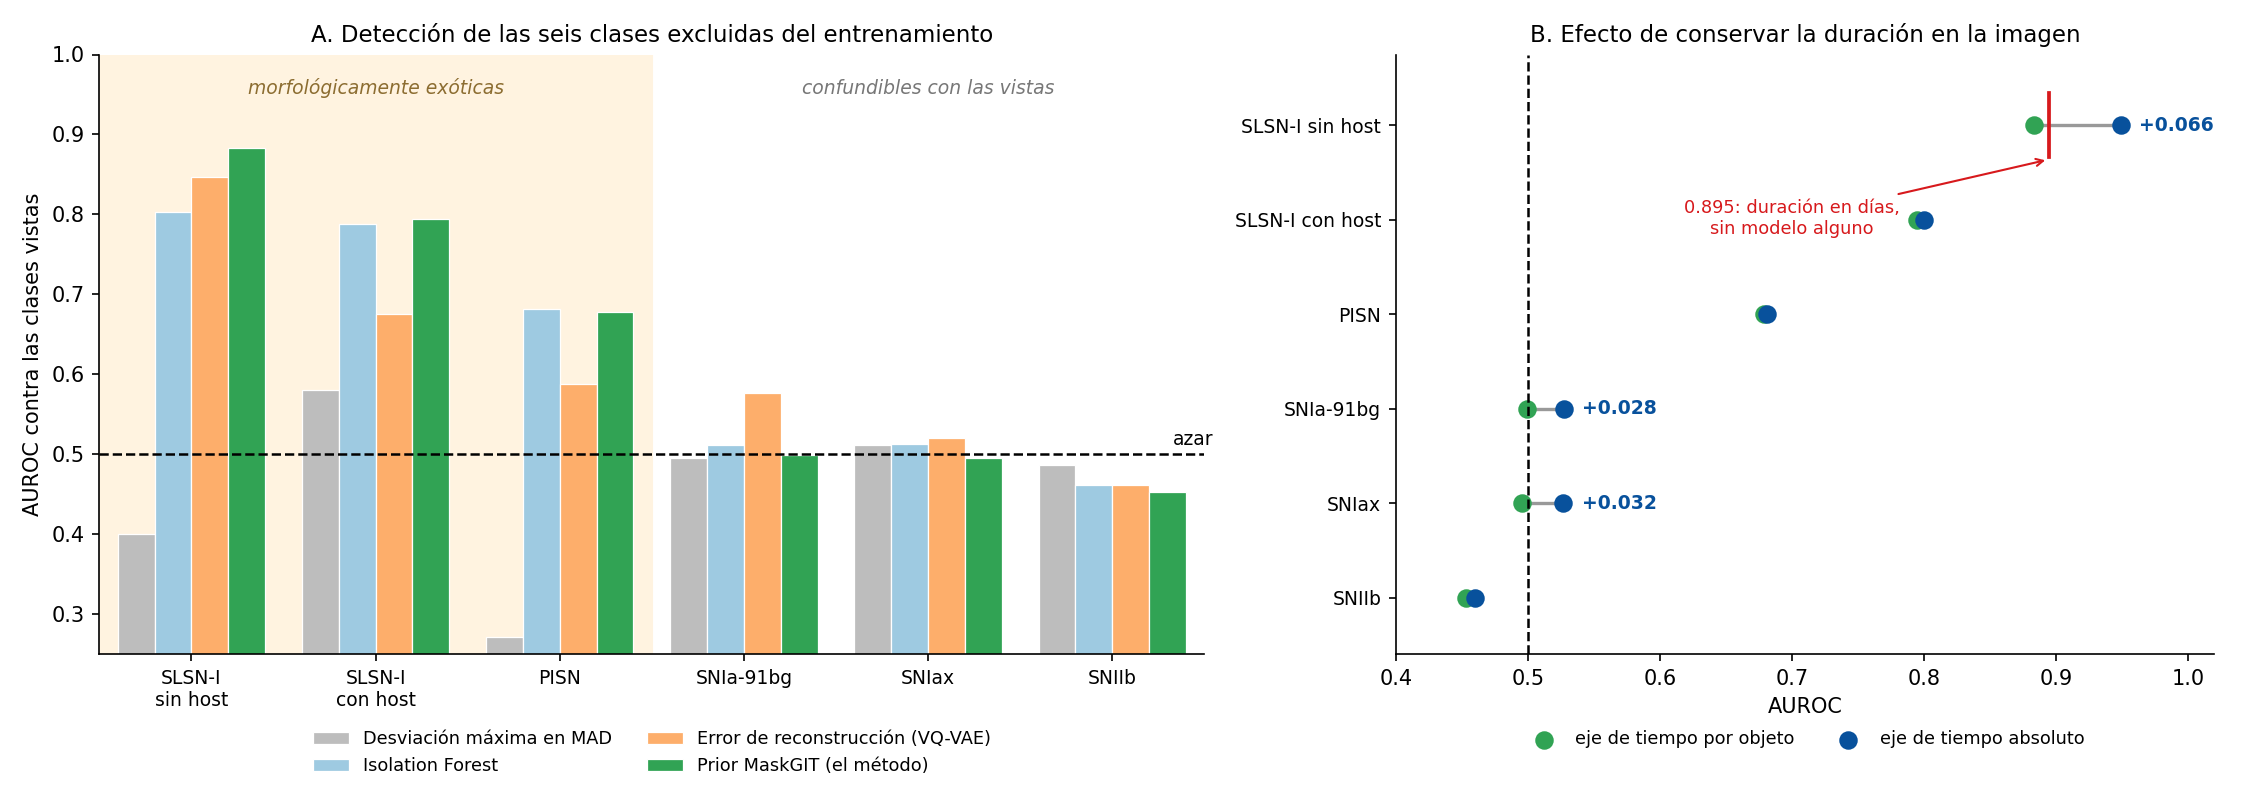
\includegraphics[width=\textwidth]{heldout_resumen.png}
\caption{Panel A: AUROC por clase y por método. La división entre las tres clases exóticas y
las tres confundibles con las vistas la respeta todo método probado. Panel B: efecto de
conservar la duración de la curva en la imagen, explicado en la última sección.}
\end{figure}

\subsection*{Lectura}

\textbf{Las seis clases se parten en dos grupos y ningún método cruza esa frontera.} En las
tres exóticas todos los métodos salvo el estadístico de una línea detectan algo, y el prior
llega a 0,883 en \texttt{SLSN-I\_no\_host}. En las tres sutiles ninguno supera 0,577 y varios
caen bajo el azar. El corte es físicamente coherente, porque \texttt{SNIax} y
\texttt{SNIa-91bg} son variantes subluminosas de las Ia y \texttt{SNIIb} transiciona hacia el
tipo Ib, así que son justamente las que se confunden con las clases vistas.

\textbf{El prior queda primero, pero por poco}, 0,634 contra 0,612 del baseline de
reconstrucción. Sobre seis clases, esa diferencia no soporta más peso que el de una
tendencia consistente.

\textbf{La elección del puntaje pesa más que la del método.} El cruce entre forma de máscara
y estadístico da:

\begin{table}[H]
\centering
\small
\begin{tabular}{@{}lcc@{}}
\toprule
\textbf{Estadístico} & \textbf{Máscara aleatoria} & \textbf{Máscara de ventana} \\
\midrule
Máximo por token          & 0,521 & 0,587 \\
Promedio de la secuencia  & 0,609 & \textbf{0,634} \\
\bottomrule
\end{tabular}
\end{table}

Entre la peor y la mejor combinación hay 0,113 de AUROC, cinco veces más que los 0,022 que
separan al prior del mejor baseline. Las dos decisiones van en la dirección esperable: el
promedio supera al máximo porque aquí lo inusual es el objeto completo y no un tramo, y la
máscara de ventana vuelve a superar a la aleatoria, igual que con anomalías sintéticas.

\section*{3. Perturbaciones más grandes en $\Delta t$}

El barrido anterior llegaba a $\Delta t = 80$ días, que sobre estas curvas cubre apenas el
32\% de los puntos de la banda \textit{r}, cuyo recorrido mediano es de unos 500 días. Se
extendió a 160 y 320 días, que cubren 58\% y 62\%.

\begin{figure}[H]
\centering
\makebox[\textwidth][c]{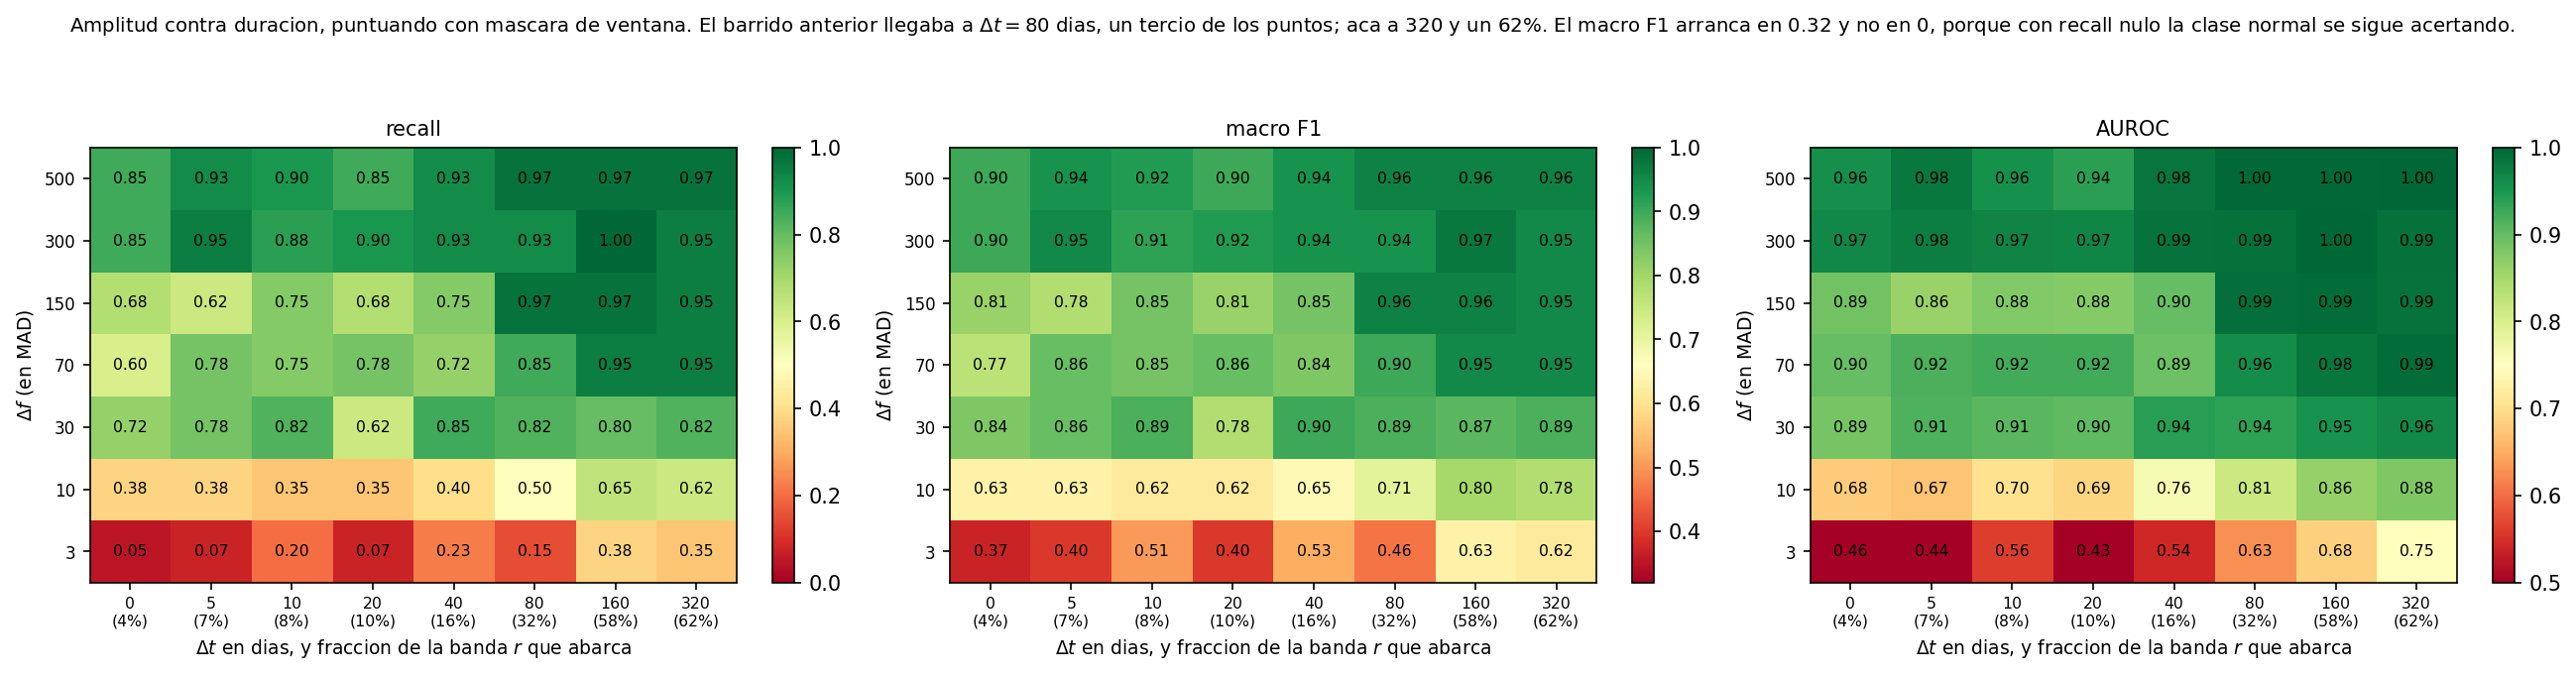
\includegraphics[width=1.16\textwidth]{barrido_duracion_folds.png}}
\caption{Recall, macro F1 y AUROC en el plano amplitud--duración, puntuando con máscara de
ventana. Entre paréntesis, la fracción de los puntos de la banda \textit{r} que abarca cada
ventana. El macro F1 usa el mismo umbral que el recall, el percentil 95 de los controles, de
modo que los falsos positivos quedan fijos en 2 de 40 por construcción.}
\end{figure}

\textbf{La detección crece en los dos ejes, pero el límite es de amplitud y no de
extensión.} Con $\Delta f = 3$ el recall no pasa de 0,38 por más que la anomalía dure 320
días, mientras que con $\Delta f \geq 300$ se detecta prácticamente siempre incluso sin
ninguna extensión temporal. Dicho de otro modo, el prior responde a cuánto se sale un punto
de lo esperable, no a cuántos puntos se salen.

\section*{4. Perturbaciones más chicas en $\Delta f$}

El barrido anterior arrancaba en $\Delta f = 10$, donde el recall ya era de 0,55, de modo que
el piso de sensibilidad quedaba fuera del rango medido. Se bajó hasta 1 MAD.

\begin{table}[H]
\centering
\small
\begin{tabular}{@{}lccccccc@{}}
\toprule
$\Delta f$ (en MAD) & 1 & 2 & 3 & 5 & 7 & 10 \\
\midrule
Exceso medio (FLUXCAL) & 5 & 9 & 14 & 23 & 33 & 47 \\
Recall & 0,12 & 0,28 & 0,33 & 0,45 & 0,53 & 0,55 \\
AUROC  & 0,493 & 0,667 & 0,715 & 0,776 & 0,794 & 0,810 \\
\bottomrule
\end{tabular}
\end{table}

\begin{figure}[H]
\centering
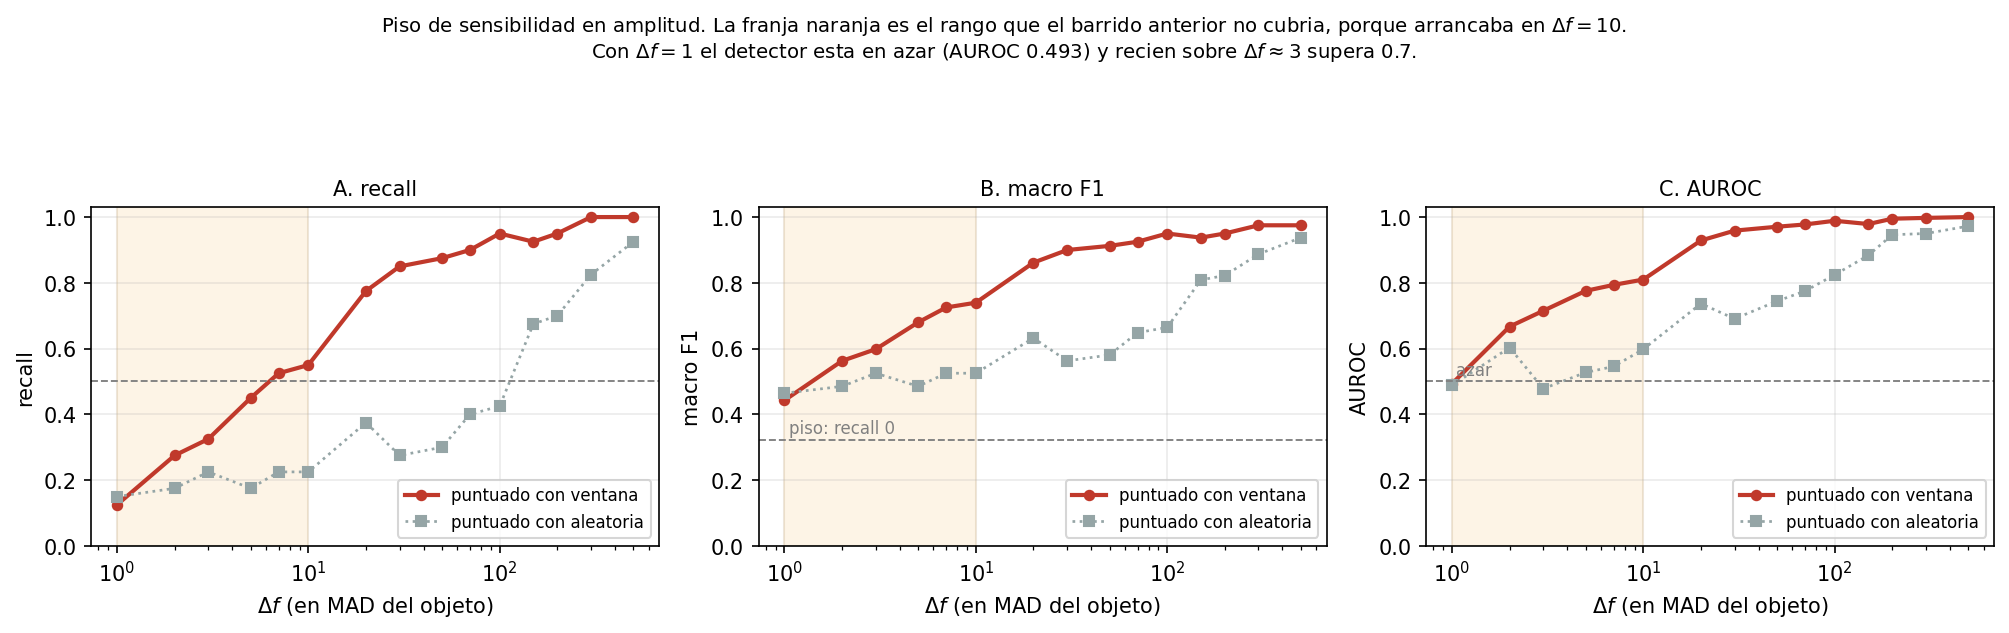
\includegraphics[width=\textwidth]{barrido_amplitud_folds.png}
\caption{Extremo inferior del barrido de amplitud, en escala logarítmica. La franja naranja
marca el rango que el barrido anterior no cubría.}
\end{figure}

\textbf{El piso queda acotado con precisión.} En $\Delta f = 1$ el AUROC es 0,493, es decir
azar exacto, que es el comportamiento que corresponde: una perturbación del tamaño de la
dispersión propia del objeto es indistinguible de esa dispersión. La separación se construye
entre 2 y 3 MAD y el recall cruza la mitad alrededor de 7 MAD, unos 33 FLUXCAL.

Un resultado secundario que vale la pena notar: puntuando con máscara aleatoria el detector
no sale del azar hasta $\Delta f = 20$. La ventaja de la máscara de ventana es entonces
\textbf{mayor justamente en el régimen de amplitudes pequeñas}, que es donde importa, y no en
el extremo donde cualquier variante funciona.

\section*{6. Imágenes variando $n$ MAD entre 5 y 300}

El parámetro es el $U$ de la codificación del flujo,

\[
u = \frac{1}{2}\left[\mathrm{clip}\left(
\frac{\operatorname{arcsinh}\left((f - \operatorname{med}(f))/\operatorname{MAD}(f)\right)}
{\operatorname{arcsinh}(U)}, -1, 1\right) + 1\right],
\]

que fija cuántos MAD entran en el carril de cada banda. Se usaron siete valores espaciados
logarítmicamente, $U \in \{5, 10, 20, 39, 77, 152, 300\}$, sobre cuatro objetos de tipos
distintos, eligiendo en cada clase el primero con fotometría en las seis bandas para que la
comparación no dependa de que falte una banda. El renderizado reproduce exactamente la
geometría del que se usa en entrenamiento.

\begin{figure}[H]
\centering
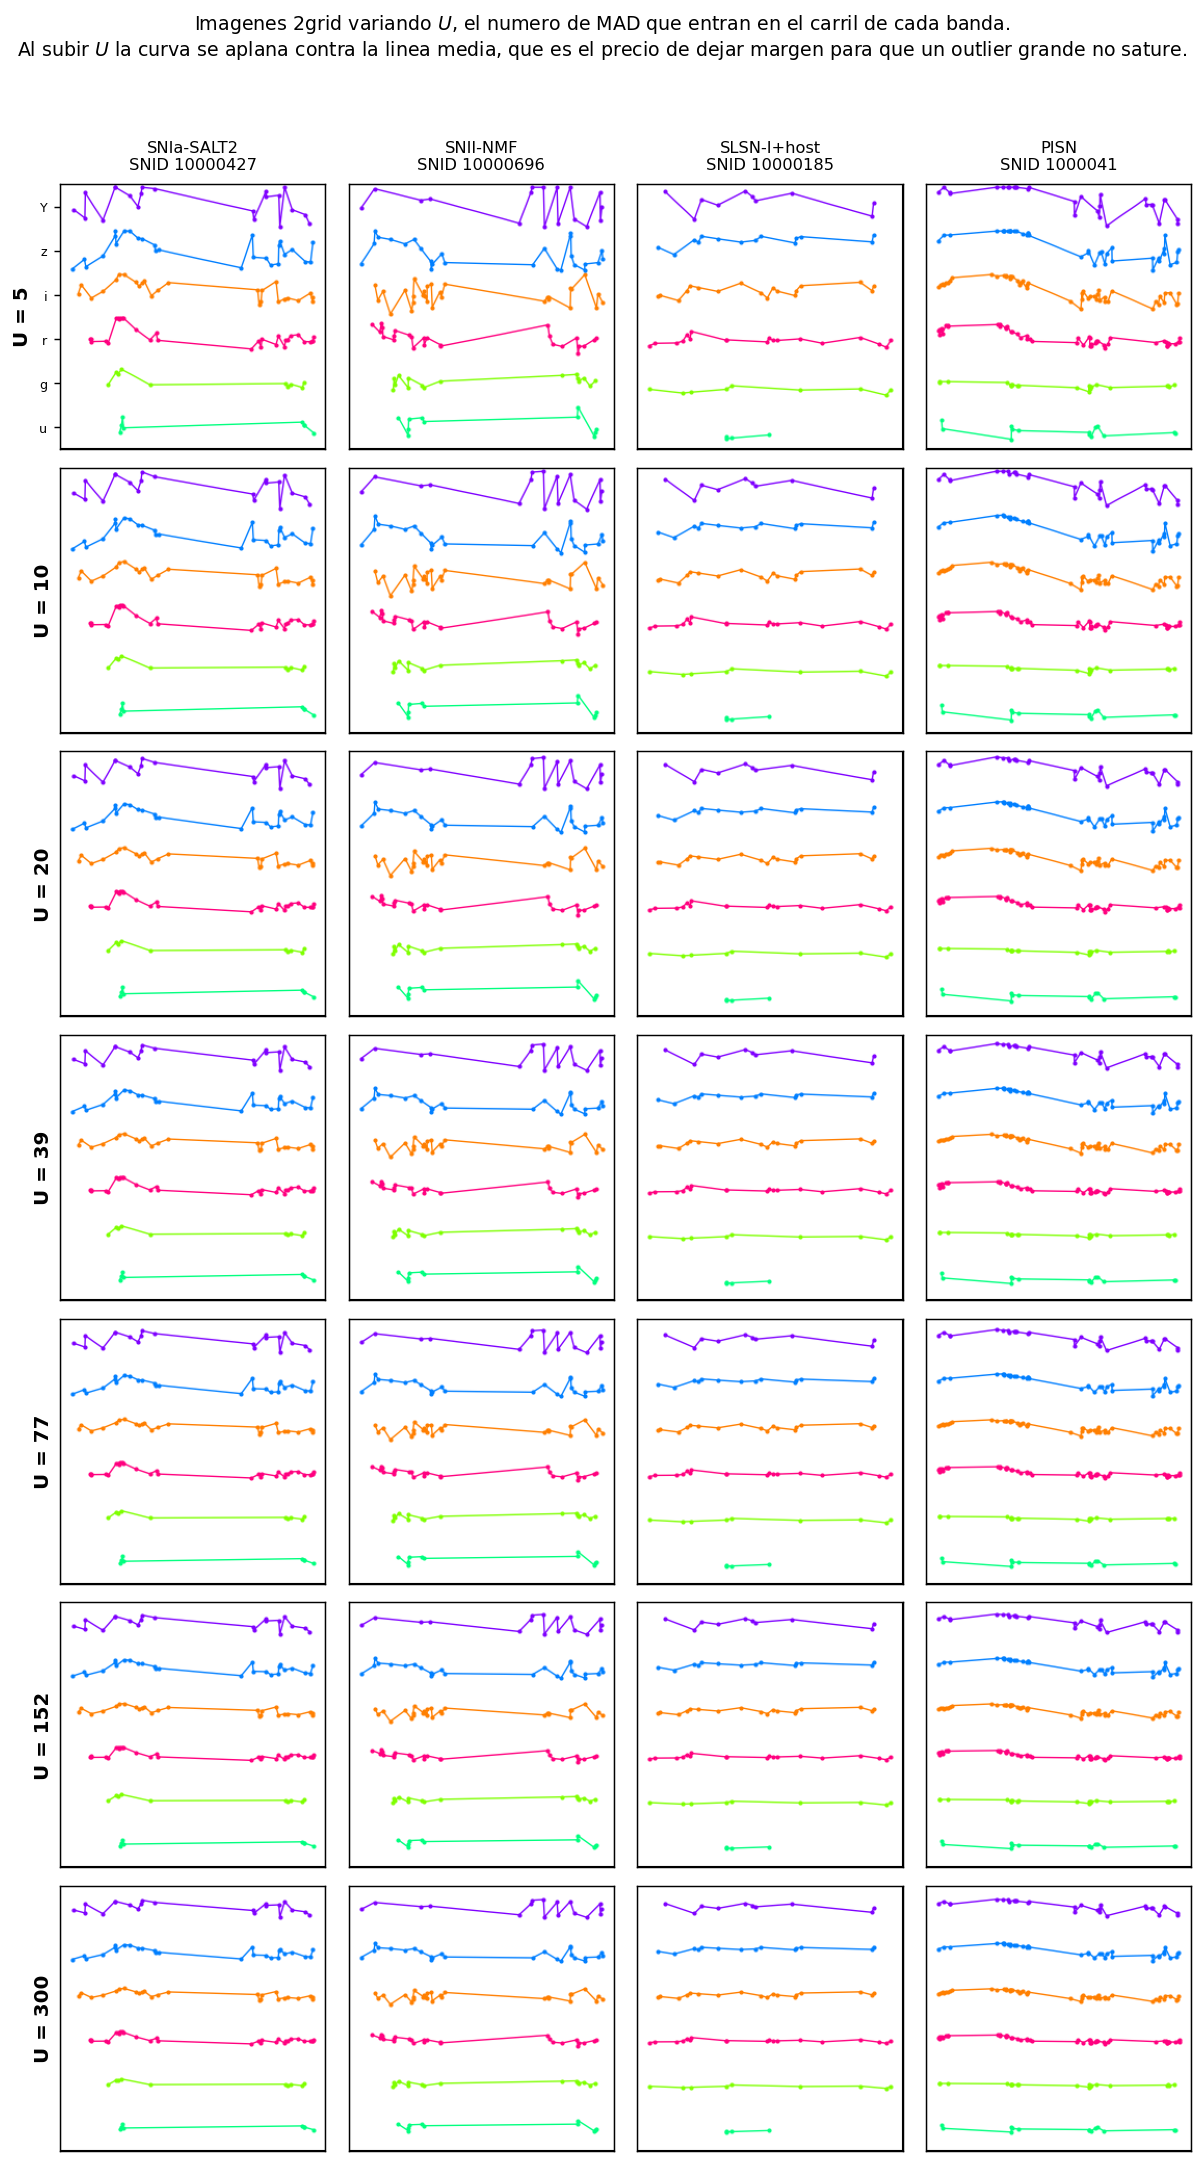
\includegraphics[height=0.74\textheight]{umad_ejemplos.png}
\caption{Imágenes 2grid variando $U$. Al subir $U$ la curva se aplana contra la línea media,
que es el precio de dejar margen para que un outlier grande no sature.}
\end{figure}

Para cuantificar el compromiso se midió qué fracción del carril ocupa realmente la curva,
tomando el rango del 90\% central:

\begin{table}[H]
\centering
\small
\begin{tabular}{@{}lcccc@{}}
\toprule
$U$ & \texttt{SNIa-SALT2} & \texttt{SNII-NMF} & \texttt{SLSN-I+host} & \texttt{PISN} \\
\midrule
5   & 0,838 & 0,919 & 0,666 & 0,809 \\
10  & 0,679 & 0,711 & 0,516 & 0,680 \\
20  & 0,553 & 0,579 & 0,420 & 0,554 \\
39  & 0,466 & 0,489 & 0,354 & 0,467 \\
77  & 0,403 & 0,422 & 0,306 & 0,404 \\
152 & 0,355 & 0,372 & 0,270 & 0,356 \\
300 & 0,317 & 0,332 & 0,241 & 0,318 \\
\bottomrule
\end{tabular}
\caption{Fracción del carril de la banda que ocupa efectivamente la curva.}
\end{table}

En $U = 300$, que es el valor adoptado, la curva normal ocupa alrededor de un tercio del
carril, y en \texttt{SLSN-I} baja a menos de un cuarto. Traducido a píxeles, con un carril
útil de 37,8 px son unos 12 px para toda la morfología de la curva, es decir
\textbf{1,5 tokens de los 4,7 que mide la banda de alto}. Esa es la explicación cuantitativa
del comentario de que las imágenes con $U = 300$ se ven planas.

\section*{Hallazgo adicional: la normalización temporal borra la señal}

Esto salió del punto 5 y terminó siendo lo más relevante del conjunto.

Para entender de dónde venía el desempeño sobre clases excluidas se midió cuánto separa cada
estadístico de la curva por sí solo:

\begin{table}[H]
\centering
\small
\begin{tabular}{@{}lcccc@{}}
\toprule
\textbf{Rasgo} & \texttt{PISN} & \texttt{SLSN-I+host} & \texttt{SLSN-I\_no\_host} &
\textbf{Fuerza media} \\
\midrule
Duración, en días  & 0,662 & 0,741 & \textbf{0,895} & \textbf{0,146} \\
Número de épocas   & 0,648 & 0,736 & 0,886 & 0,139 \\
Cadencia           & 0,634 & 0,691 & 0,811 & 0,122 \\
Brillo del pico    & 0,431 & 0,664 & 0,409 & 0,063 \\
MAD del objeto     & 0,694 & 0,625 & 0,522 & 0,068 \\
\bottomrule
\end{tabular}
\end{table}

\textbf{La duración de la curva en días, un solo número que no requiere modelo alguno,
alcanzaba 0,895 en \texttt{SLSN-I\_no\_host}, por encima del 0,883 del pipeline completo.} El
brillo absoluto, en cambio, no discriminaba, de modo que la explicación intuitiva de que las
SLSN-I se detectan por ser superluminosas quedó descartada: lo que las distingue es que duran
casi el doble.

La causa es concreta. El renderizado normalizaba el eje de tiempo dividiendo por el recorrido
observado de cada objeto, $\hat{t} = (t - t_{\min})/(t_{\max} - t_{\min})$, con lo que toda
curva ocupaba el ancho completo de la imagen y la duración desaparecía antes de que el VQ-VAE
viera nada.

\subsection*{Simetría con el problema del flujo}

Es el mismo error cometido en los dos ejes. En ambos casos la normalización por objeto se
introdujo para hacer comparables supernovas distintas, y en ambos terminó borrando
justamente lo que se quería detectar. La diferencia está en el remedio: para el flujo bastó
cambiar el estadístico, reemplazando percentiles por mediana y MAD, porque la información
seguía en la imagen y solo estaba mal escalada; para el tiempo no hay estadístico que sirva,
porque la información está directamente ausente.

\subsection*{Ablación: se reentrenó la cadena con eje temporal absoluto}

Se renderizaron de nuevo las 1.389.147 imágenes usando una escala de tiempo común de 1.110
días para todos los objetos, en vez de normalizar por el recorrido de cada uno, y se
reentrenó la cadena completa. Se eligió 1.110 días porque es apenas más que el máximo
observado, de modo que no se recorta ninguna curva. Todo lo demás se mantuvo idéntico.

\begin{figure}[H]
\centering
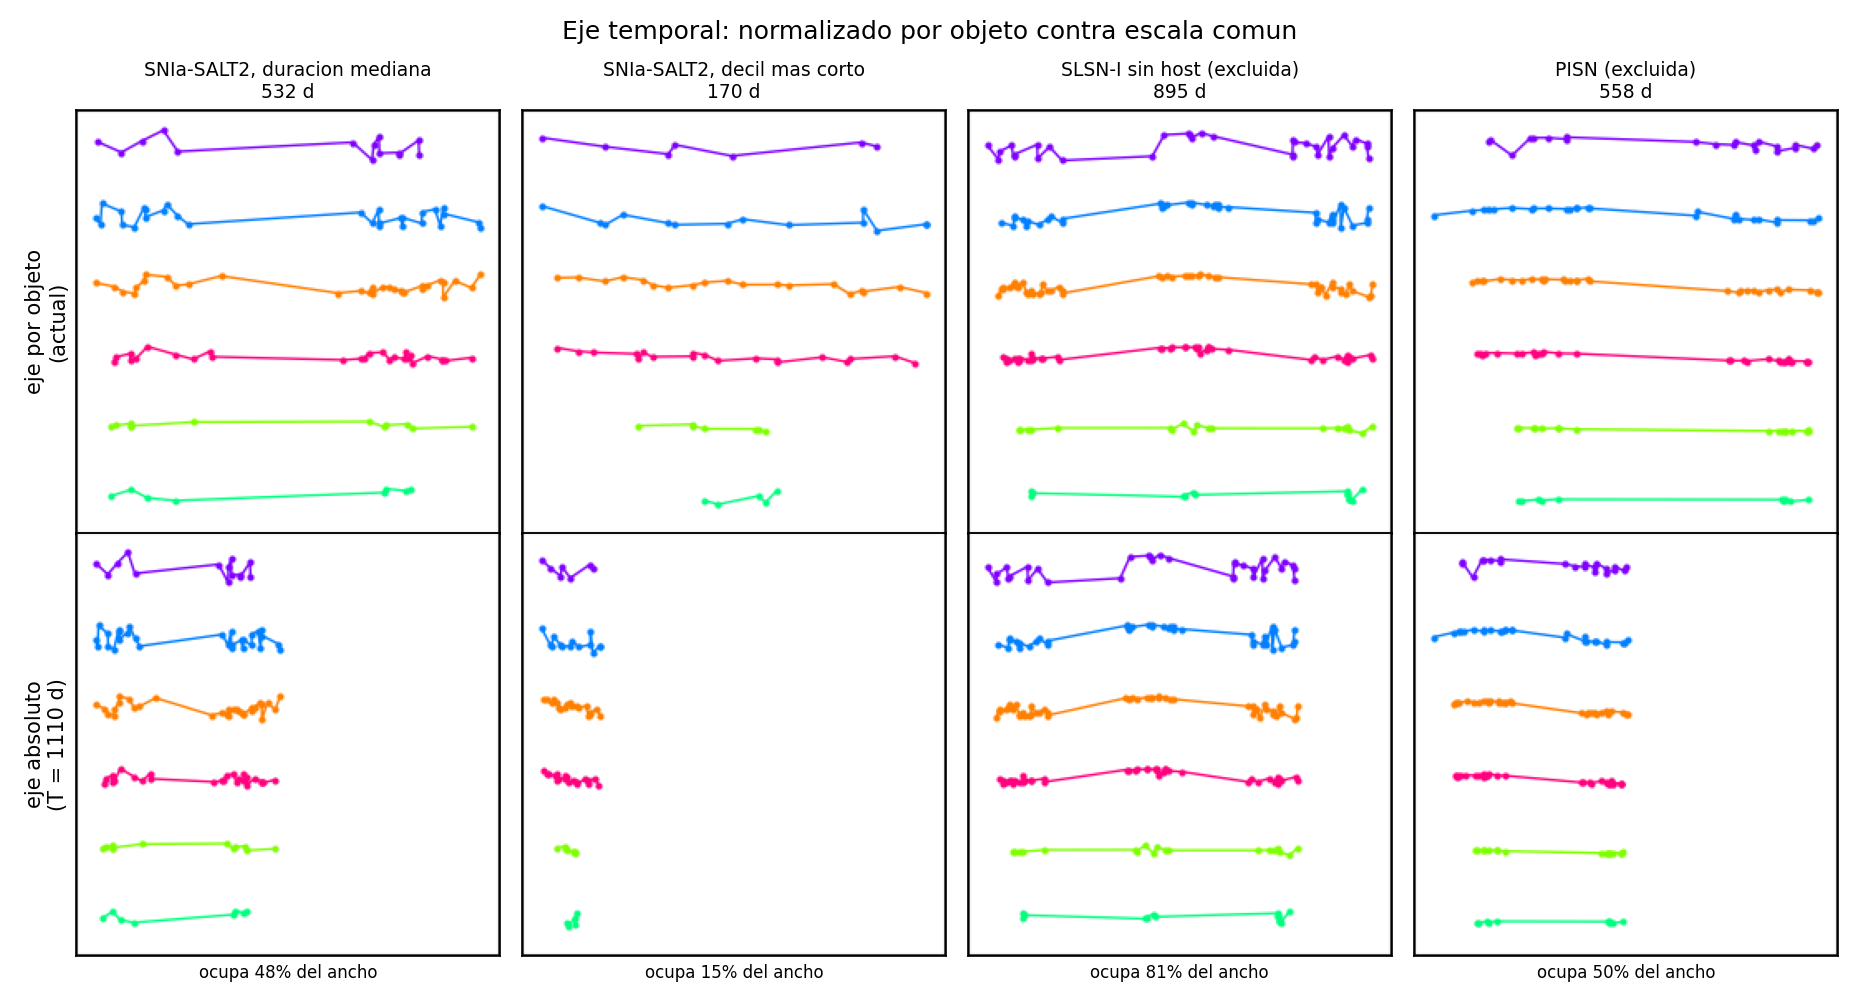
\includegraphics[width=\textwidth]{eje_temporal.png}
\caption{Los dos renderizados. Arriba el eje normalizado por objeto, donde toda curva ocupa
el ancho completo; abajo el eje absoluto, donde el ancho que ocupa la curva es su duración.}
\end{figure}

El compromiso es visible: una SLSN-I pasa a ocupar el 81\% del ancho y una SNIa corta apenas
el 15\%, es decir unos 5 tokens de los 32, con la consiguiente pérdida de resolución de
forma.

\begin{table}[H]
\centering
\small
\begin{tabular}{@{}lccc@{}}
\toprule
 & \textbf{Eje por objeto} & \textbf{Eje absoluto} & \textbf{Diferencia} \\
\midrule
\multicolumn{4}{@{}l}{\textit{Calidad de la representación}} \\
Perplexity del codebook        & \textbf{154}     & 56      & $-98$ \\
Error de reconstrucción        & \textbf{0,00223} & 0,00257 & peor \\
Exactitud del clasificador     & \textbf{0,296}   & 0,222   & $-0,074$ \\
\midrule
\multicolumn{4}{@{}l}{\textit{Detección sobre clases excluidas (AUROC)}} \\
Baseline de reconstrucción     & \textbf{0,612} & 0,600 & $-0,012$ \\
\texttt{SLSN-I\_no\_host}      & 0,883 & \textbf{0,949} & $+0,066$ \\
\texttt{SLSN-I+host}           & 0,794 & \textbf{0,800} & $+0,006$ \\
\texttt{PISN}                  & 0,679 & \textbf{0,681} & $+0,002$ \\
\texttt{SNIa-91bg}             & 0,499 & \textbf{0,527} & $+0,028$ \\
\texttt{SNIax}                 & 0,495 & \textbf{0,527} & $+0,032$ \\
\texttt{SNIIb+HostXT\_V19}     & 0,453 & \textbf{0,460} & $+0,007$ \\
\textbf{Promedio del método}   & 0,634 & \textbf{0,657} & $+0,023$ \\
\bottomrule
\end{tabular}
\caption{Efecto de conservar la duración en la imagen. La representación empeora por todas
las métricas intrínsecas y la detección mejora igual.}
\end{table}

El resultado tiene tres partes que conviene separar.

\textbf{La representación empeoró por todas las métricas intrínsecas.} La perplexity del
codebook cayó de 154 a 56 embeddings efectivos, la reconstrucción empeoró y la cabeza de
clasificación perdió exactitud. Era el riesgo previsto: con la mitad de la imagen en blanco,
buena parte de la capacidad se gasta en fondo.

\textbf{La detección mejoró de todos modos}, y lo más importante es que el baseline de
reconstrucción \textit{empeoró} en paralelo, de 0,612 a 0,600. Eso descarta que la ganancia
venga de que las imágenes sean más fáciles en general: es específicamente el prior el que
aprovecha la información nueva. En \texttt{SLSN-I\_no\_host} el pipeline pasa de 0,883 a
\textbf{0,949} y por primera vez supera con holgura al baseline de la duración sola, que era
0,895.

\textbf{Las tres clases sutiles también subieron}, poco pero las tres. Esto importa porque
era la prueba que habíamos fijado de antemano: si solo hubieran mejorado las SLSN y PISN, la
ganancia se explicaría por contar píxeles en blanco. Que suban también clases de duración
normal indica que el prior está usando algo más que el ancho. Aun así siguen cerca del azar,
en torno a 0,527, de modo que el límite de fondo sigue en pie.

\subsection*{Qué deja planteado}

La conclusión general es que, al rasterizar una serie de tiempo, cada eje que se normaliza
por objeto compra comparabilidad a cambio de descartar una variable física, y conviene
decidirlo eje por eje en vez de aplicar la misma receta a los dos por simetría. En este caso
la información descartada valía más que la capacidad de codebook que cuesta conservarla.

El objetivo pendiente queda bien definido, y no está en superar 0,80 en las SLSN-I, donde
cualquier método razonable funciona, sino en sacar algo por encima de 0,53 en
\texttt{SNIax}, \texttt{SNIa-91bg} y \texttt{SNIIb}, que son las que se confunden con las
clases normales y que hasta ahora no detecta ningún método ni ningún rasgo individual.

\end{document}
